\documentclass[12pt]{article}
\usepackage[utf8]{inputenc}
\usepackage{blindtext}
\usepackage{fancyhdr}
\usepackage{graphicx}
\usepackage{amsmath}
\usepackage{amssymb}
\usepackage{float}
  \usepackage{setspace}
\usepackage{geometry}
 \geometry{
 a4paper,
 left=20mm,
 right=20mm,
 bottom=25mm,
 top=25mm,
 }
 
 \newcommand{\icol}[1]{% inline column vector
  \left(\begin{smallmatrix}#1\end{smallmatrix}\right)%
}
 
\pagestyle{fancy}
\fancyhf{}
\lhead{Research Question:  }
\rfoot{Page \thepage}

\doublespacing
\begin{document}
\begin{titlepage}
   \begin{center}
        \vspace*{5cm}

        \Huge{Numerical Calculus for Explicit Physics Engines}

        \vspace{1cm}
        \LARGE{How can projectile motion in a computational physics engine be approximated through numerical integration?}
            
        \vspace{2 cm}
        \LARGE{\textbf{DISCONTINUED; NEVER FINISHED}}
        
        \large{(This was for my IB Math AA HL Internal Assessment, but I changed topics)}
       
       

       \vfill
    \end{center}
\end{titlepage}
    
\tableofcontents
\newpage


\section{Setting up the Physics Engine}
\subsection{Defining variables}
We will attempt to computationally simulate the projectile motion of a ball in two dimensions. Therefore, this ball is defined by its position vector, $$\vec p = \begin{pmatrix} x \\ y \\
\end{pmatrix}$$We can define the horizontal position as $x$ and vertical position as $y$. 

This ball also has velocity and acceleration acting on $x$ and $y$ with respect to time. Lets define those as $\frac{dx}{dt}$, $\frac{d^2x}{dt^2}$, respectively, for the $x$ component, and $\frac{dy}{dt}$, $\frac{d^2y}{dt^2}$, respectively, for the $y$ component. Now, what are the equations for these rates of change? 

Ultimately, we want to model the motion of a real-world ball. To begin with, lets start with a simple case with only gravity. This means that $$\frac{d^2y}{dt} = -g$$ where $g=9.81\frac{m}{s^2}$, and $\frac{d^2x}{dt} = 0$. Given that the $x$ component has no acceleration, lets first focus only on simulating the $y$ position against time.

\subsection{Numerical vs Analytical Integration}
This is a very simple differential equation that can be analytically integrated for an exact solution of $y$, as follows:

$$\frac{d^2y}{dt^2} = g \rightarrow \int \frac{d^2y}{dt} dt = \int g dt \rightarrow \frac{dy}{dt} = gt + y_0 \rightarrow \int \frac{dy}{dt} dt = \int (gt + v_{y0}) dt$$
$$\therefore y = \frac{1}{2} gt^2 + v_{y0} t + y_0 $$

This solution has its merits: its \textit{exact} and easy to compute. However, it is very limited in a physics engine because it assumes acceleration is constant, which is not always the case (and will not be once we add bounce and drag to the simulation). Moreover, this equation is not true to how objects move: a ball in the real world does not compute how much time has passed since its existence to know where it will be next; rather, it has instantaneous rates of change that move it ever so slightly in tiny time-steps. This calls for numerical integration, which we have seen before in this course with the Euler method. Numerical integration is not exact: it is an approximation. This means that it will need optimization to accurately simulate a moving ball. This investigation's focus is to find the most computationally efficient method for best approximating this projectile motion. 

\section{Exploring Numerical Integration Methods}

\subsection{Taylor Expansion}
To numerically integrate acceleration, we must find a differential equation for velocity and position with respect to time. We can use a Taylor series to approximate a solution for these two variables. For clarity, lets define the function $y(t)$ as the position of $y$ at time $t$ of the simulation and $v_y(t)$ as the rate of change of $y$ at time $t$. At time $t$, both variables are defined from the previous time-step already, so this notion of time is abstracted from us. However, in finding the amount these values changed over a time-step $\Delta t$, it helps to think of them as a function of time. 
$$v(t+\Delta t) = v(t) + \Delta t v^\prime(t) + \frac{\Delta t^2}{2}v^{\prime \prime}(t) + ...$$

$$y(t+\Delta t) = y(t) + \Delta t y^\prime(t) + \frac{\Delta t^2}{2}y^{\prime \prime}(t) + ...$$

Although with only gravity many of the terms in this infinite series are zero, lets generalize this to future cases where the ball may have a fourth derivative, fifth, sixth, etc. In that case, we will never know the value of the infinite series, so let's approximate it by taking the first two terms. Now, we can substitute out this abstract notion of time for the current position/ velocity of the object to find the new values after timestep $\Delta t$. 
$$\frac{dy}{dt}_{next} \approx \frac{dy}{dt} + \Delta t \frac{d^2y}{dt^2}$$
$$y_{next} \approx y + \Delta t \frac{dy}{dt}$$

\subsection{Euler Method}
By approximating the Taylor Expansion, we can now apply the Euler Method to numerically integrate this. Think of each frame in the computer as the time-step (more precisely, the inverse of the frame-rate). If standard video games compute 30 frames per second, then our time-step for the Euler method is $\Delta t = \frac{1}{30}.$ The smaller the time-step, the closer our approximation is to the analytically integrated equation for position. 

$$\Delta t = \frac{1}{framerate} = \frac{1}{30}s$$

This got me thinking, how can we decrease the time-step without increasing the frame-rate? Since the computer runs each 'step' every time it loops through the code, I realized the only way to lower $\Delta t$ was to embed a double Euler by introducing a second time-step, $h$. Now, the actual step is even lower than the frame-rate: in fact it is $\Delta t \times h$. I implemented both into my code in Figure 1 to see how both would do against the analytically solved exact integration for the moving ball.

\begin{figure}[H]
\centering
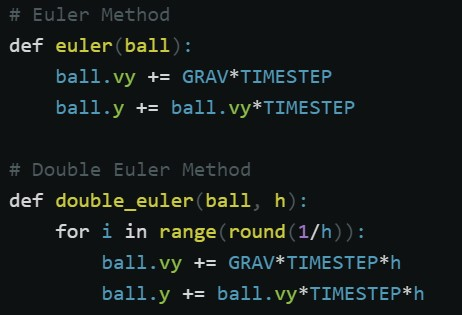
\includegraphics[width=200pt]{img/euler_code.jpg}
\caption{\label{fig:1}My Euler Method Code}
\end{figure}

Now, let's see how these results compare to the ideal equation for projectile motion derived above. Using my own python program, the NumPy data science package, and MatPlotLib data visualization package, I obtained the following graph for the first 0.1 seconds using a framerate of 30 frames per second and a second timestep of 0.2 for the double euler. In terms of computational complexity, $\zeta$ (how many calculations are necessary to simulate the physics engine), we have the following values: 
$$\zeta_{Euler} = \frac{1}{\frac{1}{30}} = 30 \; \frac{computations}{second}$$
$$\zeta_{Double-Euler} = \frac{1}{\frac{1}{30} \times 0.2} = 150 \; \frac{computations}{second}$$
Clearly the Double-Euler is extremely computationally heavy, so this is a less desired option unless it proves the only method to increase precision.

\begin{figure}[H]
\centering
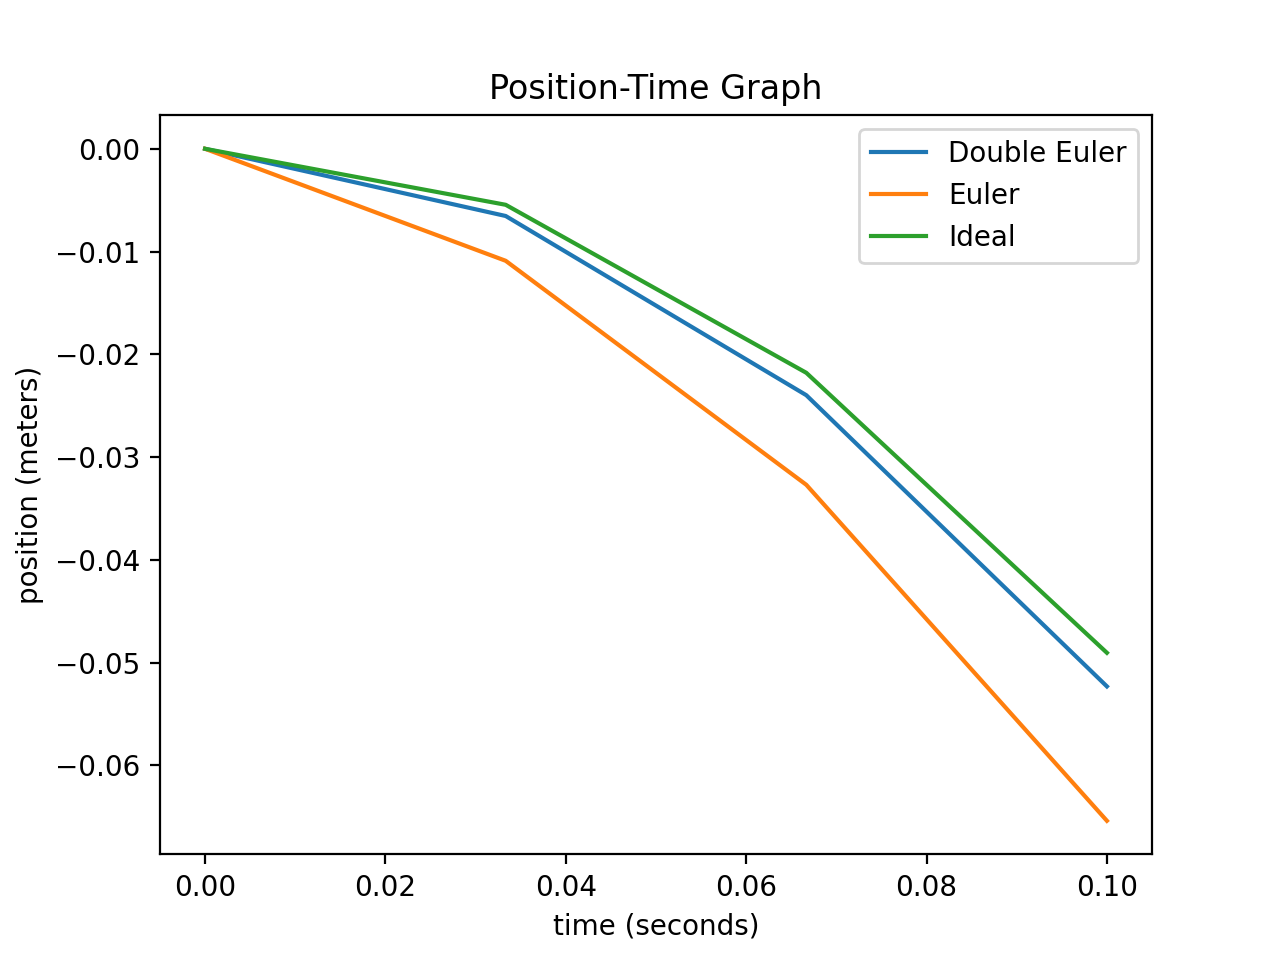
\includegraphics[width=300pt]{img/euler.png}
\caption{\label{fig:1}Free Fall Graph using Euler Method}
\end{figure}

The ball was set to an initial velocity vector of $\vec 0$ and set into free fall. The exact equation is represented with the green 'ideal' line. The orange line, the Euler method with a timestep of $\frac{1}{30}s$, is farthest off. In fact, the first computed value is twice the position of the ideal equation. This is simply shown by comparing both equations, 
$$g(1) = 2 \times \frac{1}{2}g(1)^2$$

Therefore, the Euler method with a timestep inverse of the framerate is an inadequate representation of a ball undergoing projectile motion. However, the double euler is far closer, yet it also increasingly deviates, and is extremely computationally heavy. 

\subsection{Runge-Kutta Method}

The previous results were either extremely inaccurate or extremely computationally heavy: neither works for a physics engine which needs to be accurate and optimized. While researching for other methods for numerical integration, I found that the industry-standard method used by most game studios is the fourth order Runge-Kutta method. 

The Runge-Kutta method approximates the differential equation:
$$\frac{dy}{dt} = f(t,y(t)), \; y(t_0) = y_0$$
Using:
$$y_{n+1} = y_n + \frac{h(k_1+2k_2+2k_3+k_4)}{6}$$
Where
$$k_1 = f(t_n,y_n)$$
$$k_2 = f(t_n+\frac{h}{2},y_n + h\frac{k_1}{2})$$
$$k_3 = f(t_n+\frac{h}{2},y_n + h\frac{k_2}{2})$$
$$k_4 = f(t_n+h,y_n+hk_3)$$

In our current simple scenario of an object in free fall, $f(t,y)$ is substituted with the previously derived second-order approximations for position and velocity based on the Taylor Expansion. 

Amazingly, when I ran the Runge-Kutta-4 method on my code, it approximated the ideal line almost perfectly. After $0.1s$ as in the previous, trial, it measured the ball in the exact same position as the ideal equation: $-0.0490m$. To see when the difference would accumulate, I ran the same test for $10,000s$. Even then, the error was $6.25\times 10^{-13}m$ at a position of $-490.5m$, meaning it was off by
$$\Delta RK4 = \frac{Ideal_{peak} - RK4_{peak}}{Ideal_{peak}} = \frac{6.25\times 10^{-13}}{490.5} \approx (1.27 \times 10^{-15})\%$$ 
That is such an insignificant difference that we can confidently add more factors to the projectile motion to further approximate a real-life bouncing ball.

\section{Introducing Perfectly Elastic Bounce}

Let's add a floor at $0m$ to the simulation, at which point the ball will bounce in the opposite direction. Importantly, we will \textbf{not} introduce a loss in energy at each bounce, meaning that the collision is perfectly elastic and it should reach the same peak height each time it bounces. 

In terms of mechanics, a vertical bounce is a reorientation of the velocity vector from the direction $\theta$ to $360 - \theta$. Using a conditional statement, we can now add a line of code to the simulation stating 

$$\text{if } y \le 0 \text{ then } \frac{dy}{dt}_{next} = \frac{dy}{dt} \times -1$$

While in theory this condition should suffice for a bounce mechanism, some trials would have the balls stuck below the ground as they did not have sufficient velocity to escape the floor and enter a perpetual cycle of going slightly up, then down. To solve this, I implemented the absolute value function instead, as any bounce on the floor will result in a positive velocity.

$$\text{if } y \le 0 \text{ then } \frac{dy}{dt}_{next} = \mid \frac{dy}{dt} \mid$$

This fixed the bug and can be seen in the following figure. 

\begin{figure}[H]
\centering
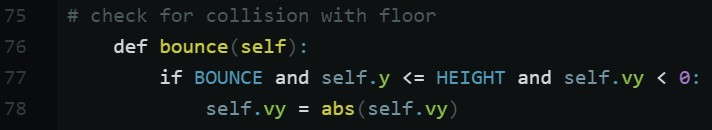
\includegraphics[width=300pt]{img/bounce_code.jpg}
\caption{\label{fig:1}}
\end{figure}

Note how bouncing immediately takes away our ability to explicitly integrate the velocity vector to find the position vector of the ball, as every time it bounces a new differential equation arises. From here on out, we are limited to only the Euler, double Euler, and RK4 numerical integration methods. However, we already verified that the RK4 method is extremely accurate, so we can have certainty that it will approximate the motion correctly. As a result, we will continue using the three numerical integration methods as we continue complicating the simulation to compare them, thus assess how accurate the RK4 is in relative to the Euler Method. 

Since the ball will bounce, let's initialize the ball with a velocity of $\frac{dy}{dt} = 5$. This way the ball starts off by going upwards, then bounces.

\begin{figure}[H]
\centering
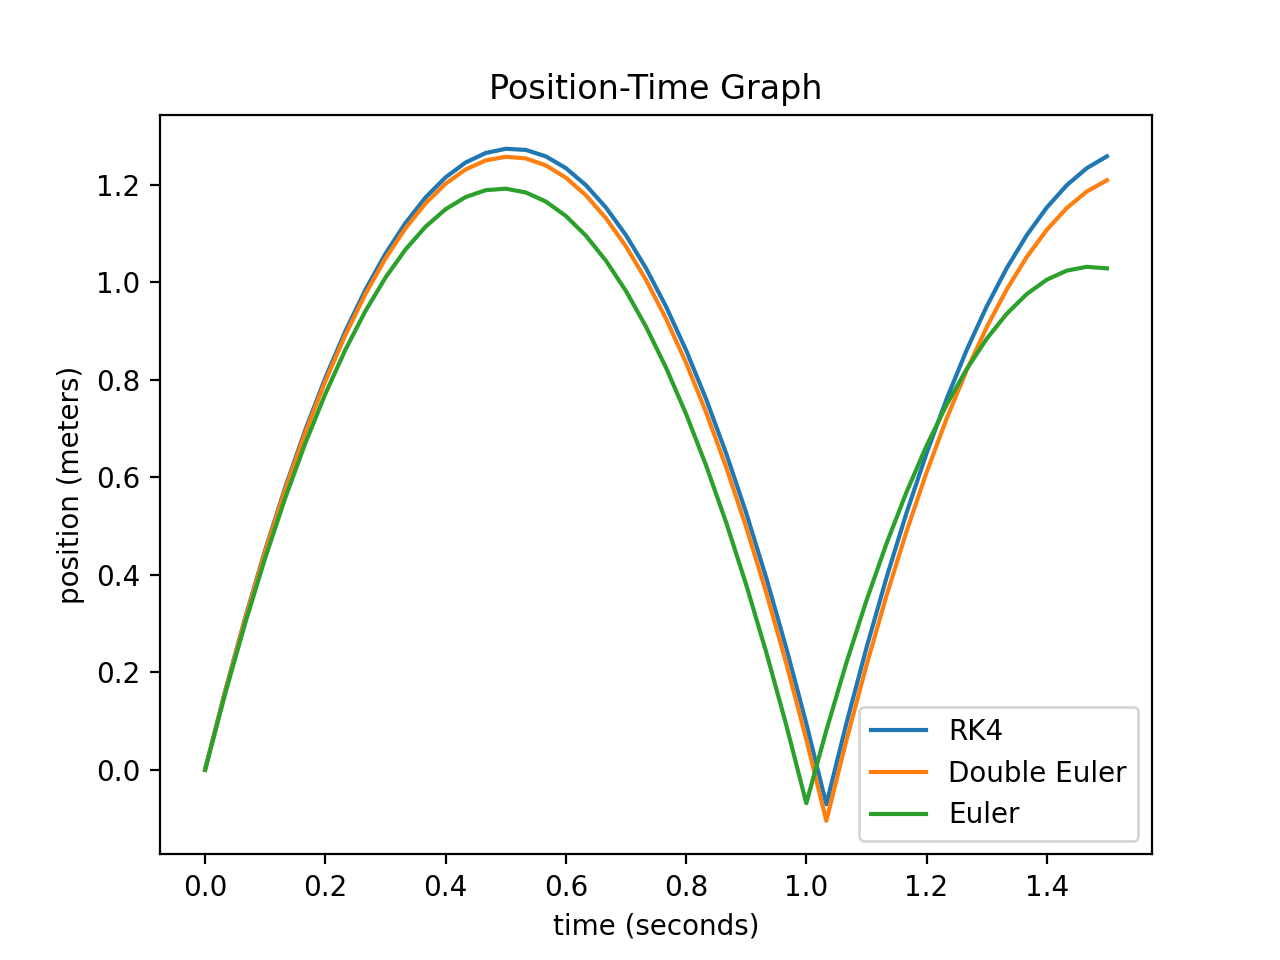
\includegraphics[width=300pt]{img/one_and_half.png}
\caption{\label{fig:1}}
\end{figure}

This is the position-time graph after $1.5$ seconds. Something really interesting happens here, because the difference gradually accumulates over time until the peak position at around $1.5$ seconds is much lower for the Euler Method green and orange lines. However, the blue line, representing the RK4 method, maintains the same peak of about $1.03m$. This is an interesting failure of the Euler Method, so let's increase the timestep to $6$ seconds. 

\begin{figure}[H]
\centering
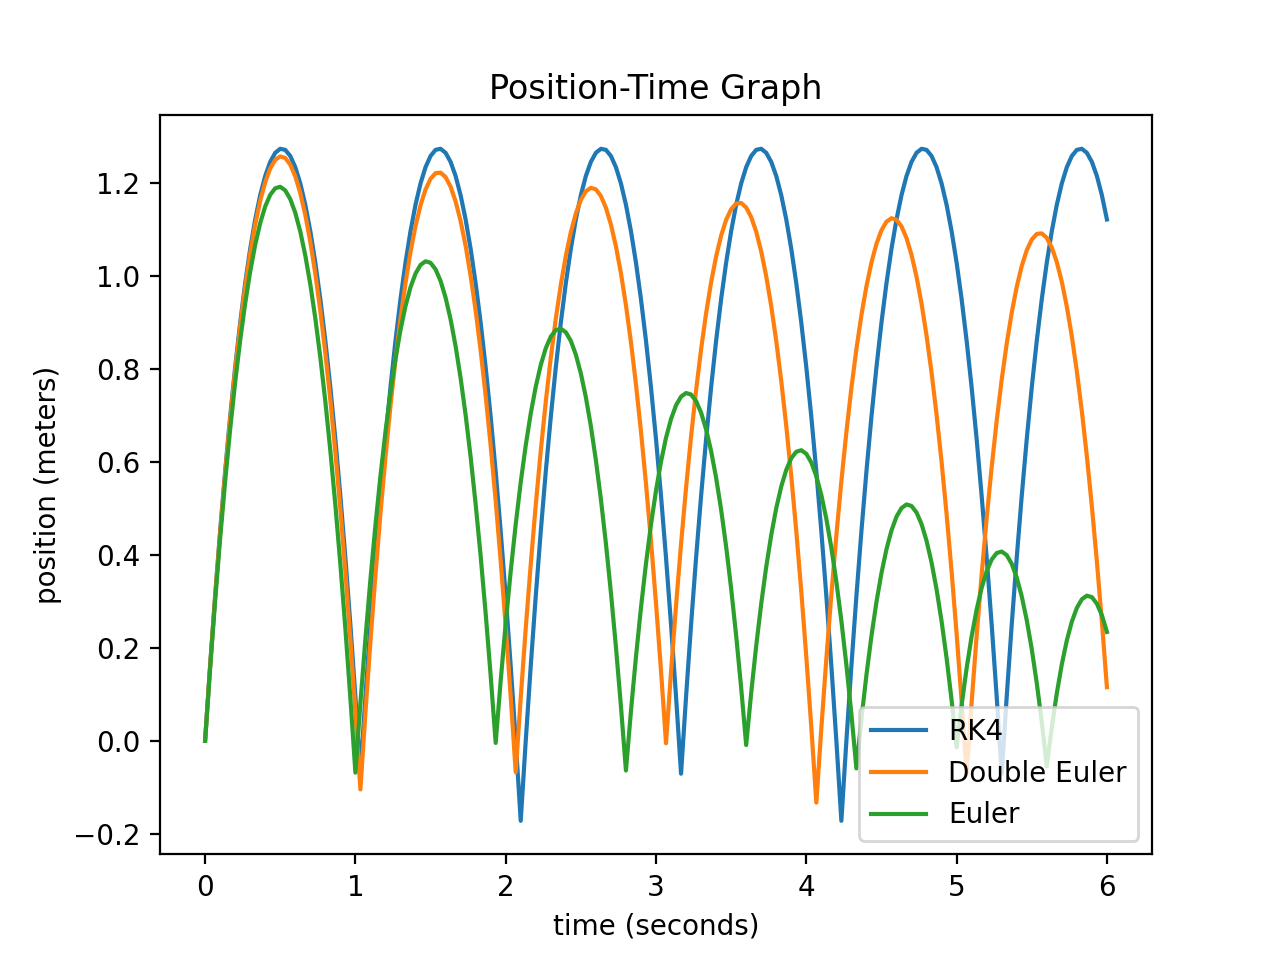
\includegraphics[width=300pt]{img/energy_loss.png}
\caption{\label{fig:1}}
\end{figure}

The position-time graph demonstrates how the Euler Method is slowly decreasing its peak height, where the larger the timestep the slower this decrease occurs. Nonetheless, even the Double Euler, running 150 computations per frame, decreases by 
$$\frac{y_{Double-Euler}}{y_{RK4}} = \frac{0.115}{1.12} \approx 10.3\%$$

in just 6 seconds. I wondered whether this pattern would continue until the ball comes to rest, so I increased the time to 150 seconds. 

\begin{figure}[H]
\centering
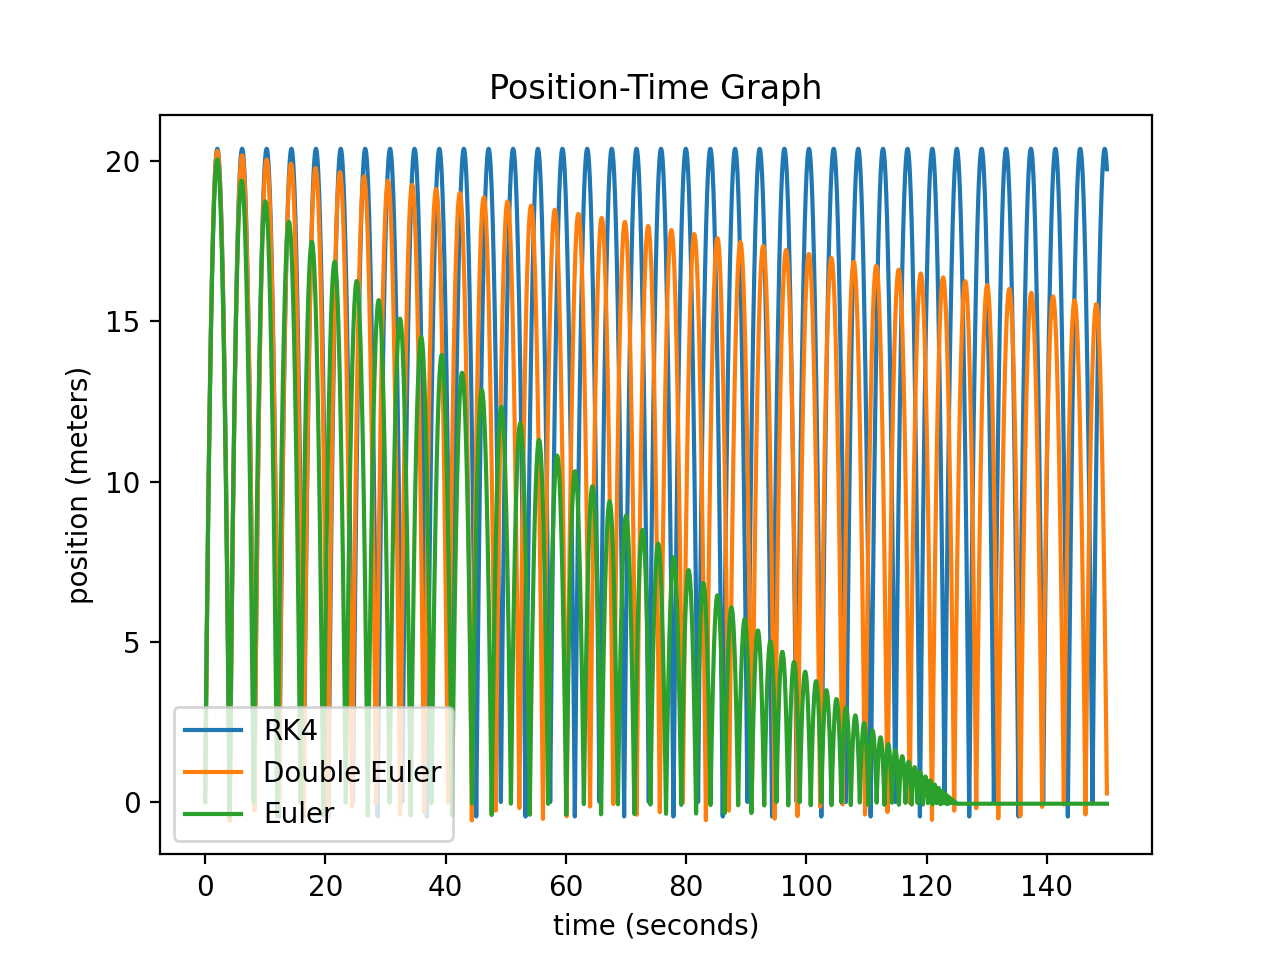
\includegraphics[width=300pt]{img/super_long.png}
\caption{\label{fig:1}}
\end{figure}

This graph shows how the RK4 method maintains precise energy conservation as the peak height remains the same, while the Euler linearly decreases. Clearly, this indicates that the Euler Method can not be maintained in a simulation or physics engine running for medium to long periods of time.

To quantify this difference beyond the visual appeal of Figure 5, the following is a graph of the path-differences of each integration method across time. 

\begin{figure}[H]
\centering
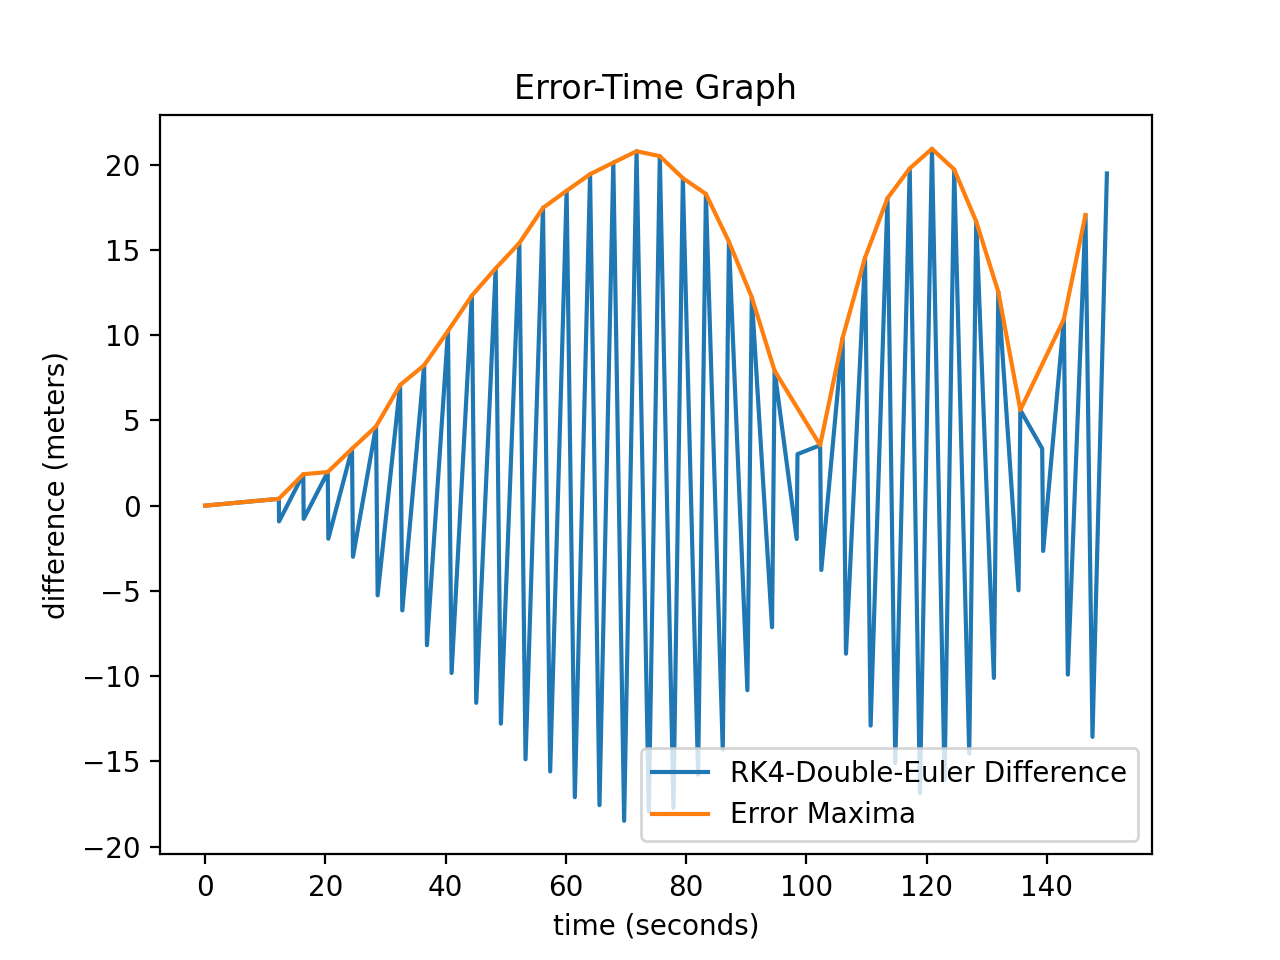
\includegraphics[width=300pt]{img/long_error.png}
\caption{\label{fig:1}}
\end{figure}

The blue line represents the difference in position between the Double-Euler Method and the RK4 Method. This error accumulates over time until about 70 seconds, then decreases until another peak is reached. This error visualization highlights an almost sinosodial relationship between error and time. To highlight this, I programmed my own algorithm using the SciPy signal processing package that passes through each local maxima of the blue line. This line demonstrates how as the balls bounce, the Euler Method has sinosodial maximum error with decreasing frequency, meaning that the maximum error repeats increasingly faster. This orange line confirms that the Euler Method, even with a large timestep, is too inaccurate compared to the RK4 Method.

\section{Introducing Drag} 

Now that we know with certainty that the Runge-Kutta-4 method will approximate projectile motion more accurately than the Euler and double Euler, let's further complicate the simulation to better simulate a real-life bouncing ball by adding air resistance.

\subsection{Defining the ODE}
According to SOURCE, air resistance minimizes the acceleration of an object proportionally to its velocity squared. This gives us the following equations, 
$$\frac{d^2y}{dt^2} = g - kv_y^2 \qquad \qquad \qquad \frac{d^2x}{dt^2} = - kv_x^2$$
Where $k$ is the drag coefficient, otherwise dependent on mass, area, and other currently insignificant factors, that have been abstracted out of this point-mass investigation. I will temporarily set the drag coefficient to $k=0.5$ to have a noticeable impact on the position of the ball.

However, there is still a problem. Drag makes acceleration smaller, so it would be untrue to always subtract it. Instead, it should be subtracted from acceleration when the velocity is positive, and added when velocity is negative, so that velocity always decreases. At first, I wanted to solve this using an 'if-else' statement in the code of the simulation. However, I found that the ODE can be modified instead to the following, more accurate, representation of drag, where velocity squared is modified to velocity times its absolute value, thus opposing the direction of velocity, 
$$\frac{d^2y}{dt^2} = g - k \mid v_y \mid v_y \qquad \qquad \qquad \frac{d^2x}{dt^2} = - k \mid v_x \mid v_x$$

Now we can apply this to the Euler and Double Euler Method using the previous Taylor Expansion, resulting in the following implementation: 



After defining $\frac{dy}{dt}$ and $\frac{dx}{dt}$ from the above equation, I now had to implement the Runge-Kutta Method. I did so using the same approach as before but for both the $x$ and $y$ directions, resulting in the following code: 

\begin{figure}[H]
\centering
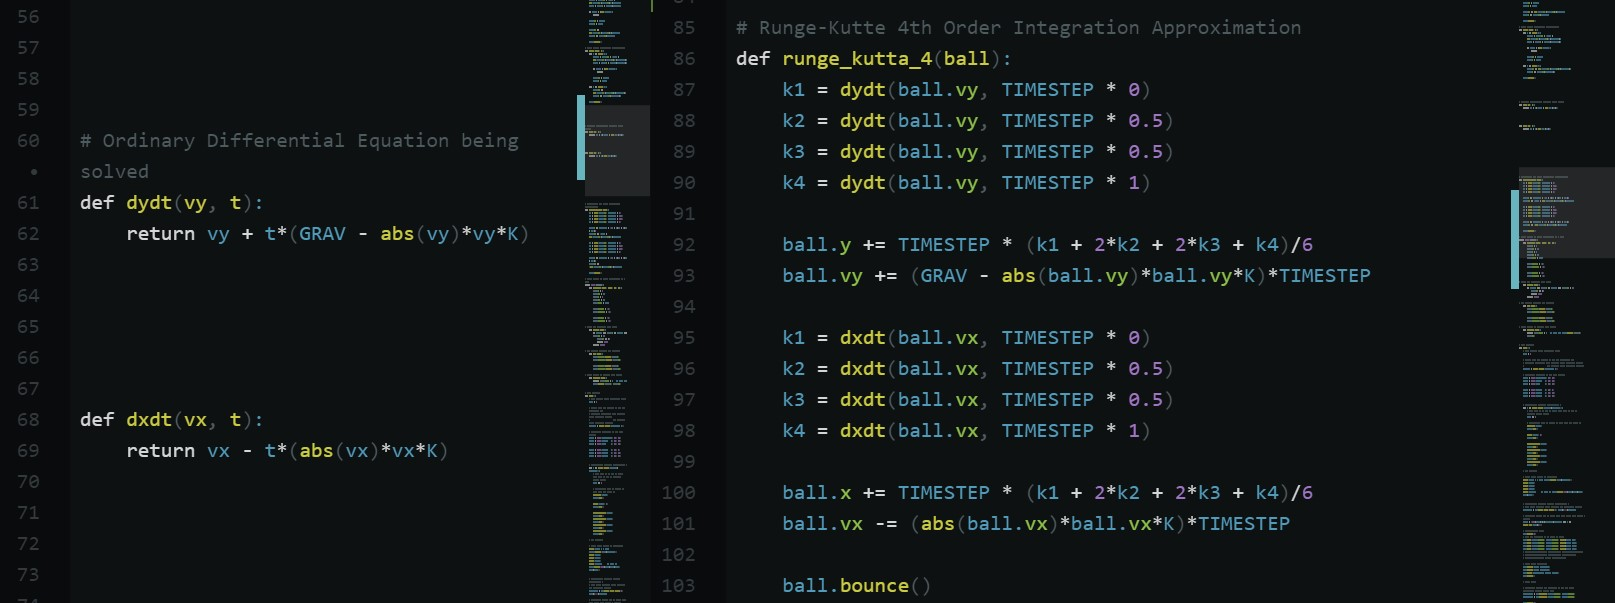
\includegraphics[width=500pt]{img/RK4_code.jpg}
\caption{\label{fig:1}}
\end{figure}

\subsection{Assessing Results}

We can now plot x-position versus y-position as opposted to position versus time since both component vectors are acted upon by air resistance. The following is what our graph looks like after $1.5$ seconds.

\begin{figure}[H]
\centering
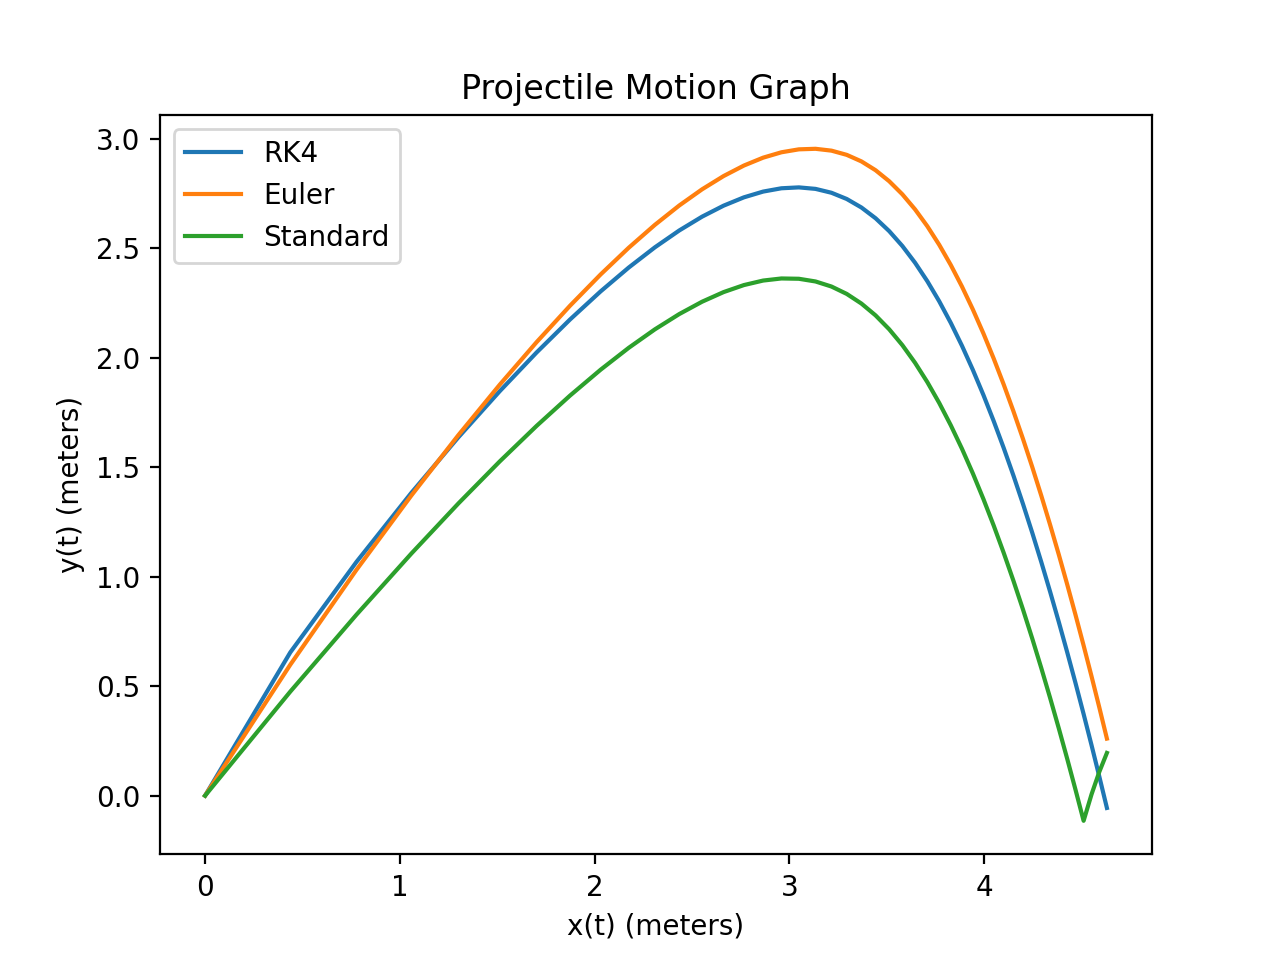
\includegraphics[width=300pt]{img/air_1.png}
\caption{\label{fig:1}}
\end{figure}

This is interesting, because the Double Euler actually estimates a higher peak height for the ball compared to the RK4. This would indicate that the RK4 method actually performed poorer in the short-term, possibly because of the 150 versus 4 computations per frame of the double euler compared to the RK4. This would suggest that the double euler indeed best approximates the motion for this more complex motion of a ball through air. 

\subsection{Maintaining Long-Term Behavior}

However, this is no longer the case when we observe long-term behavior. Despite under-calculating the peak height, the RK4 method better conserves energy over time, as shown before. The same result appears with air resistance, as show n in the figure below. 

\begin{figure}[H]
\centering
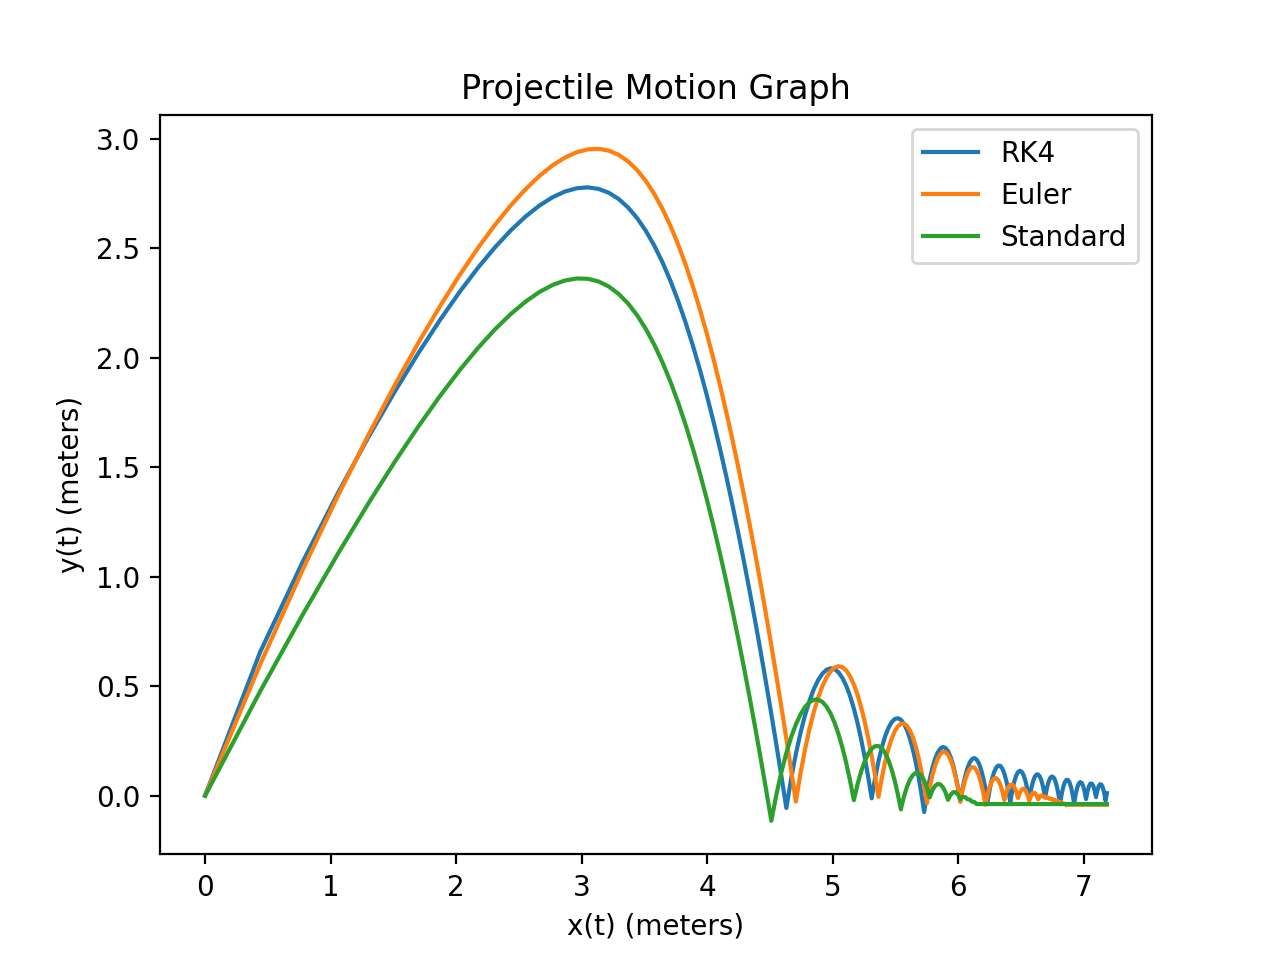
\includegraphics[width=300pt]{img/air_2.png}
\caption{\label{fig:1}}
\end{figure}

This indicates that although a lower peak height is approximated, the RK4 method better approximates the motion of a bouncing ball through air resistance over longer periods of time, like $6$ seconds or more. Here, the Euler and Double Euler both reach rest after just a few seconds, while the RK4 continues to bounce, better resembling real-life bouncing mechanics. 

Let's confirm this observation by examining the error graph of difference in position between the Double Euler and RK4 over time. 

\begin{figure}[H]
\centering
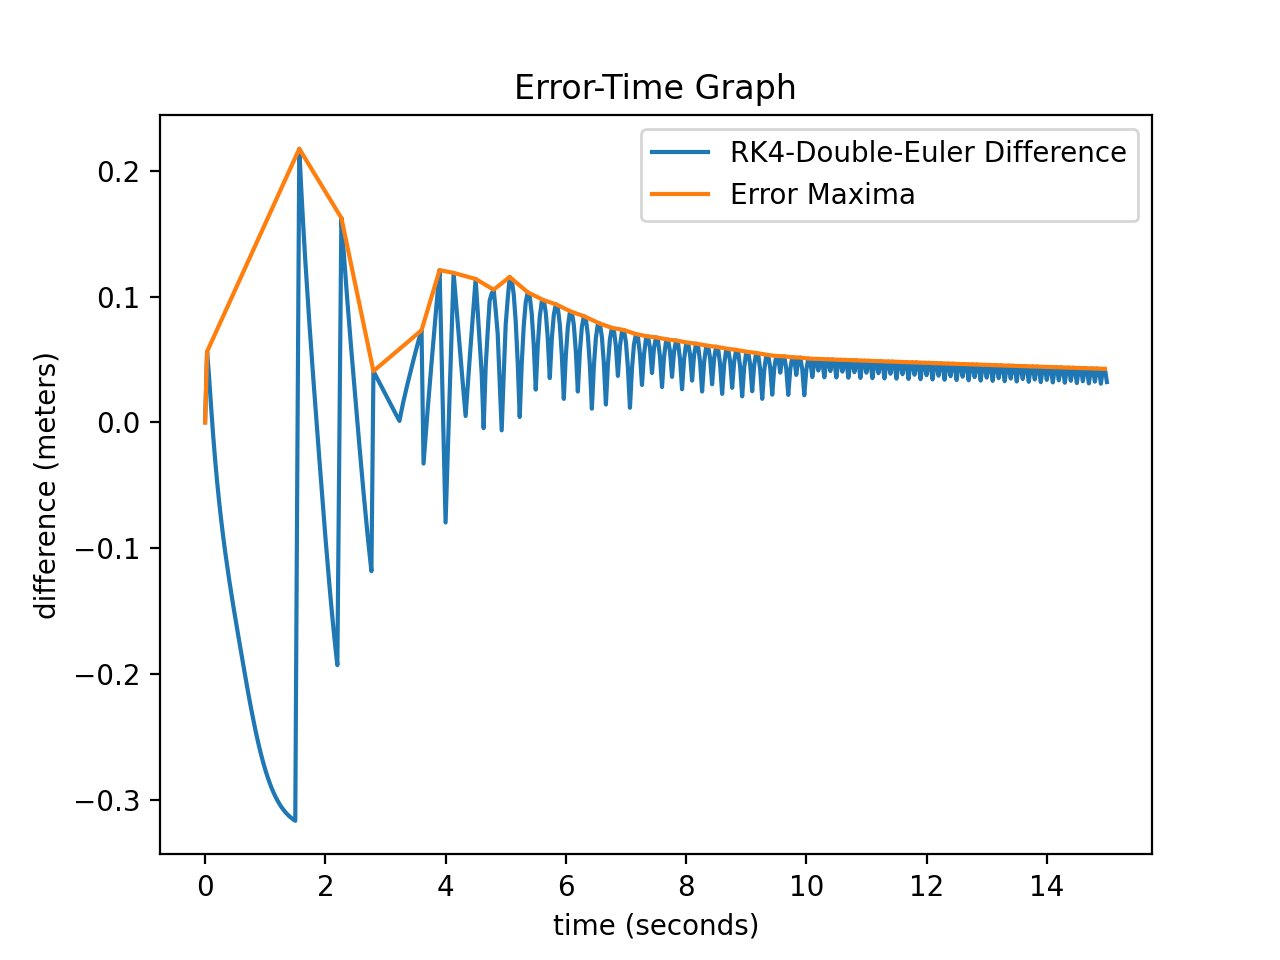
\includegraphics[width=300pt]{img/drag_error.png}
\caption{\label{fig:1}}
\end{figure}

Interestingly, the error graph now observes the pattern of an initial spike, after which it generally decreases over time, especially in the time period 5 seconds to 10 seconds. I similarly applied my local-maxima algorithm to the graph, illustrated in orange. This indicates that with air resistance, the difference between both integration methods decreases rapidly over time. However, crucially as observed in Figure 8, the integration methods of the Euler and Double Euler reach rest at around 0 meters after only 6 and 7 seconds, respectively. Therefore, even with air resistance, the RK4 method more accurately approximates the real-life movement of a bouncing ball through air resistance.

Now that these results were confirmed, I lowered the drag coefficient to a more realistic number like $k=0.1$. Furthermore, I wanted to test this across multiple values, so I created test trials with varying velocity vectors: 

$$
\begin{pmatrix} \frac{dx}{dt} \\ \frac{dy}{dt} \\
\end{pmatrix} = 
\begin{pmatrix} 15 \\ 5 \\
\end{pmatrix}, 
\begin{pmatrix} 15 \\ 10 \\
\end{pmatrix}, 
\begin{pmatrix} 15 \\ 25 \\
\end{pmatrix}, 
\begin{pmatrix} 15 \\ 80 \\
\end{pmatrix}
$$

This yields the following results:
\begin{figure}[H]
\centering
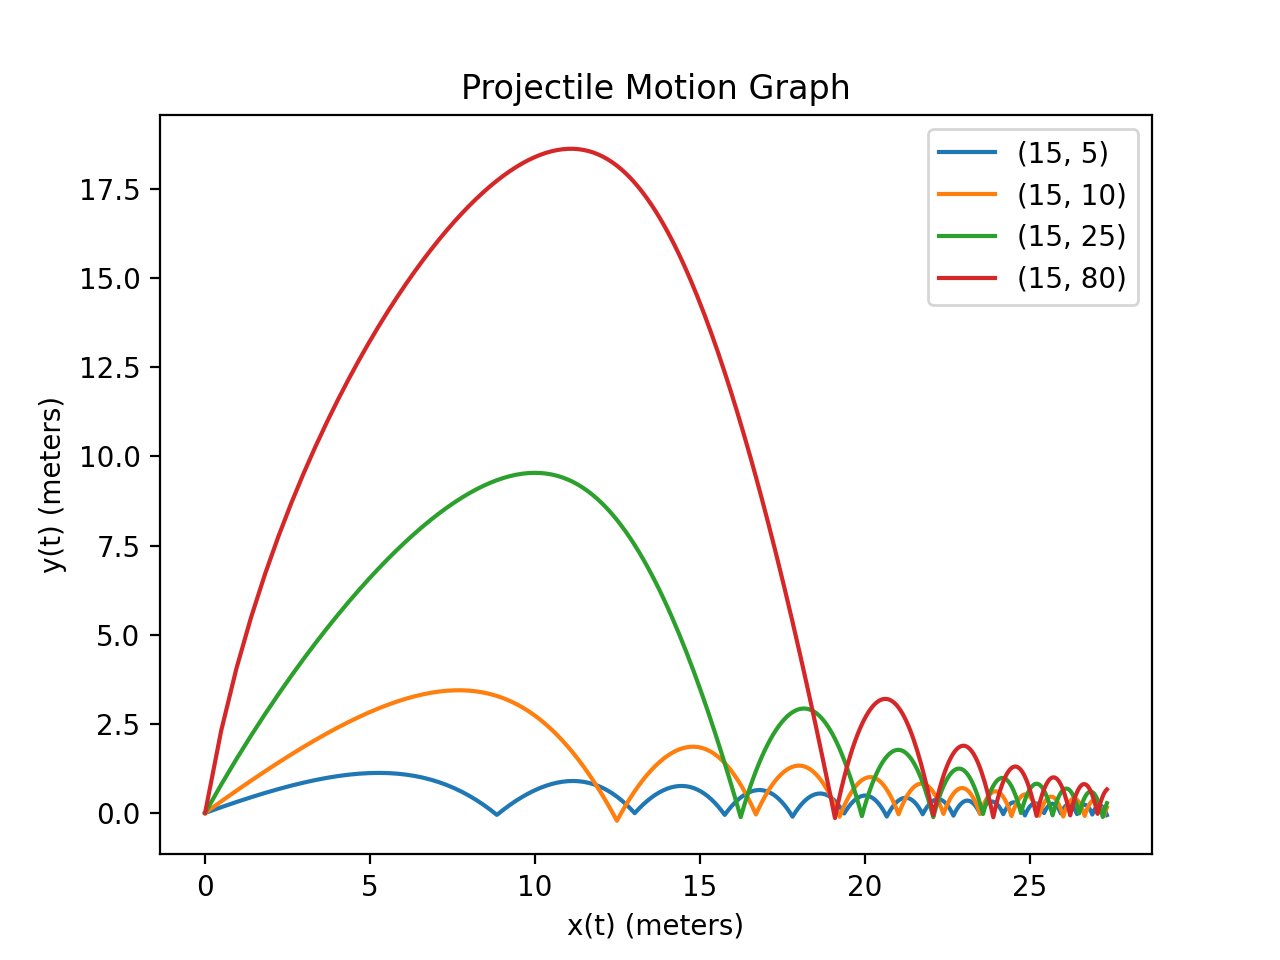
\includegraphics[width=300pt]{img/multiple.png}
\caption{\label{fig:1}}
\end{figure}

This demonstrates how varrying initial velocity vectors affect the trajectory of a bouncing ball through air resistance. In all cases, the motion behaves in line with what would be expected from a real-life projectile.

\section{Conclusion}

Ultimately, the Runge-Kutta Method seems to be both the most computationally efficient and numerically accurate. 

While the Euler Method is good at approximating the motion with a smaller timeste, as shown with the conistently more accurate results of the double-euler, this is incredibly computationally costly and will not suffice for large-scale videogames or complex simulations. If, for example, this code were to be used to approximate the motion of a thousand interacting molecules, that means that a thousand computations have to be done per second, multiplied 

\section{Applications}

Numerical integration has direct application to videogames. For any objects to be rendered as they move, the Runge-Kutta Method is commonly employed

\section{Extensions}
An important extension would be to explore other numerical integration methods to approximate the projectile motion of the ball. While less prominent than the Runge-Kutta Method, there are other methods including The Midpoint Rule, The Trapezoidal Rule, and Simpson's Rule. Each vary in accuracy and computational complexity, meaning that they could potentially achieve even better results than the RK4. 

Another extension would be to add more forces to the simulation to make it more realistic. This could include dissipation of energy every time the ball bounces, leading to realistic loss of mechanical energy. Spring forces could also be added, allowing the ball to compress when bouncing. 

\end{document}
